\documentclass[border=3pt,tikz]{standalone}
\usetikzlibrary{calc}


\begin{document}
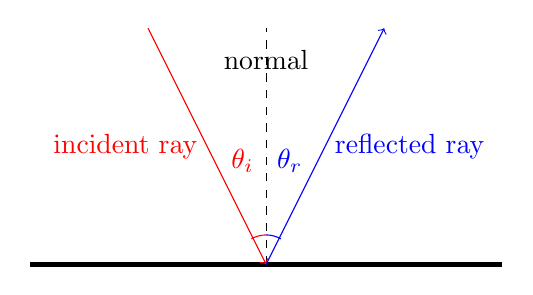
\begin{tikzpicture}
    % Draw the mirror
    \draw[ultra thick] (0,0) -- (6,0);
    
    % Draw the normal
    \draw[dashed] (3,0) -- (3,3);
    
    % Draw the incident ray
    \draw[red,->] (1.5,3) -- (3,0);
    
    % Draw the reflected ray
    \draw[blue,->] (3,0) -- (4.5,3);
    
    % Draw the angle arcs
    \draw[red] (3,0.375) arc (90:120:0.375);
    \draw[blue] (3,0.375) arc (90:60:0.375);
    % Label the normal
    \node[] at (3,2.6) {normal};
    
    % Label the incident ray
    \node[red,left] at (2.25,1.5) {incident ray};
    
    % Label the reflected ray
    \node[blue,right] at (3.75,1.5) {reflected ray};
    
    % Label the angles
    \node[red] at ($(3,0)+(120:0.6)+(0.0,0.8)$) {$\theta_i$};
    \node[blue] at ($(3,0)+(60:0.6)+(-0.0,0.8)$) {$\theta_r$};
\end{tikzpicture}
\end{document}

